\documentclass[12pt]{article}
\usepackage[
  paperheight=4.25in, 
  paperwidth=5.5in,
  margin=.4in
]{geometry}
\usepackage{tikz}

\def\headsize{0.4}
\def\elevatorwidth{2.5}

\tikzstyle{person}=[ultra thick, orange!50, scale=0.8]

\tikzset{
  elevator/.pic = {
    \draw[fill=gray!30] 
      (-.2,-.05) rectangle (\elevatorwidth+.2,4.05);
    \draw[fill=white] 
      (0,0) rectangle (\elevatorwidth,4);

    %guide-line (for development)
    %\draw (\elevatorwidth/2,0) -- ++(0,4);


    \path (\elevatorwidth/2,4.4) coordinate (pulley);
    \draw (pulley) -- ++(0,-0.4);
    \filldraw[fill=gray] (pulley) circle (0.3);
    \filldraw[fill=gray!50] (pulley) circle (0.2);
    \draw[thick] (pulley) 
      ++(-0.3,1) --
      ++(0,-1)
      arc[start angle=-180, end angle=0, radius=0.3] --
      ++(0,1);
  }
}




\begin{document}
\pagestyle{empty}

\begin{center}
  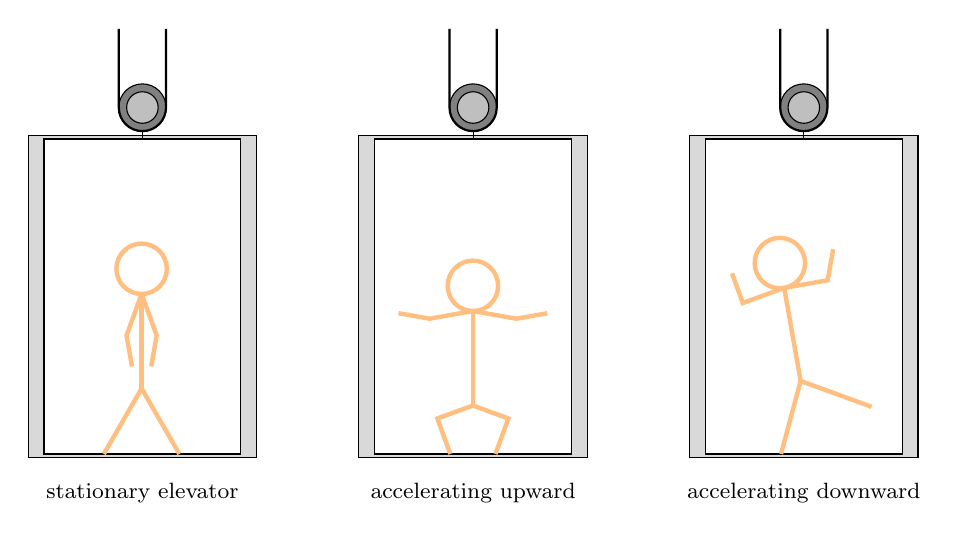
\begin{tikzpicture}

    \begin{scope}
      \path (0,0) pic{elevator} coordinate (start);

      \begin{scope}[person]
        \draw (start) 
        ++(.95,0) coordinate (left foot) --
        ++(60:1.2) coordinate (waist) --
        ++(-60:1.2) coordinate (right foot);

        \draw (waist)
          -- ++(90:1.5) coordinate (neck);
        \draw (neck) 
          ++(90:\headsize) circle (\headsize);
        \draw (neck)
          -- ++(-70:0.7) coordinate (right elbow)
          -- ++(-100:0.5) coordinate (right hand);
        \draw (neck)
          -- ++(-110:0.7) coordinate (left elbow)
          -- ++(-80:0.5) coordinate (left hand);
      \end{scope}

      \draw (start) ++(\elevatorwidth/2,-0.5)
        node {\footnotesize stationary elevator};

    \end{scope}

    \begin{scope}
      \path (4.2,0) pic{elevator} coordinate (start);


      \begin{scope}[person]
        \draw (start) 
        ++(1.2,0) coordinate (left foot) --
        ++(110:0.6) --
        ++(20:0.6) coordinate (waist) --
        ++(-20:0.6) --
        ++(250:0.6) coordinate (right foot);


        \draw (waist)
          -- ++(90:1.5) coordinate (neck);
        \draw (neck) 
          ++(90:\headsize) circle (\headsize);
        \draw (neck)
          -- ++(-10:0.7) coordinate (right elbow)
          -- ++(10:0.5) coordinate (right hand);
        \draw (neck)
          -- ++(190:0.7) coordinate (left elbow)
          -- ++(170:0.5) coordinate (left hand);
      \end{scope}

      \draw (start) ++(\elevatorwidth/2,-0.5)
        node {\footnotesize accelerating upward};

    \end{scope}

    \begin{scope}
      \path (8.4,0) pic{elevator} coordinate (start);

      \begin{scope}[person]
        \draw (start) 
        ++(1.2,0) coordinate (left foot) --
        ++(75:1.2) coordinate (waist) --
        ++(-20:1.2) coordinate (right foot);

        \draw (waist)
          -- ++(100:1.5) coordinate (neck);
        \draw (neck) 
          ++(100:\headsize) circle (\headsize);
        \draw (neck)
          -- ++(10:0.7) coordinate (right elbow)
          -- ++(80:0.5) coordinate (right hand);
        \draw (neck)
          -- ++(-160:0.7) coordinate (left elbow)
          -- ++(110:0.5) coordinate (left hand);
      \end{scope}

      \draw (start) ++(\elevatorwidth/2,-0.5)
        node {\footnotesize accelerating downward};

    \end{scope}

  \end{tikzpicture}
\end{center}

\end{document}